\documentclass[border=10pt]{standalone}
\usepackage[T1]{fontenc}
\usepackage{tikz}
\usetikzlibrary{matrix, calc}
\usepackage{tgheros} % For a sans-serif font similar to the header

% Define colors from the image
\definecolor{headerblue}{HTML}{B0D0E8}
\definecolor{rowblue}{HTML}{E6F0F7}
\definecolor{orgblue}{HTML}{C9E3F2}
\definecolor{headertextblue}{HTML}{0077BE}
\definecolor{statuscritical}{HTML}{FF7F50}
\definecolor{statusendangered}{HTML}{2E8B57}
\definecolor{statusthreatened}{HTML}{0077BE}
\definecolor{statusvulnerable}{HTML}{3C78B4}

\begin{document}
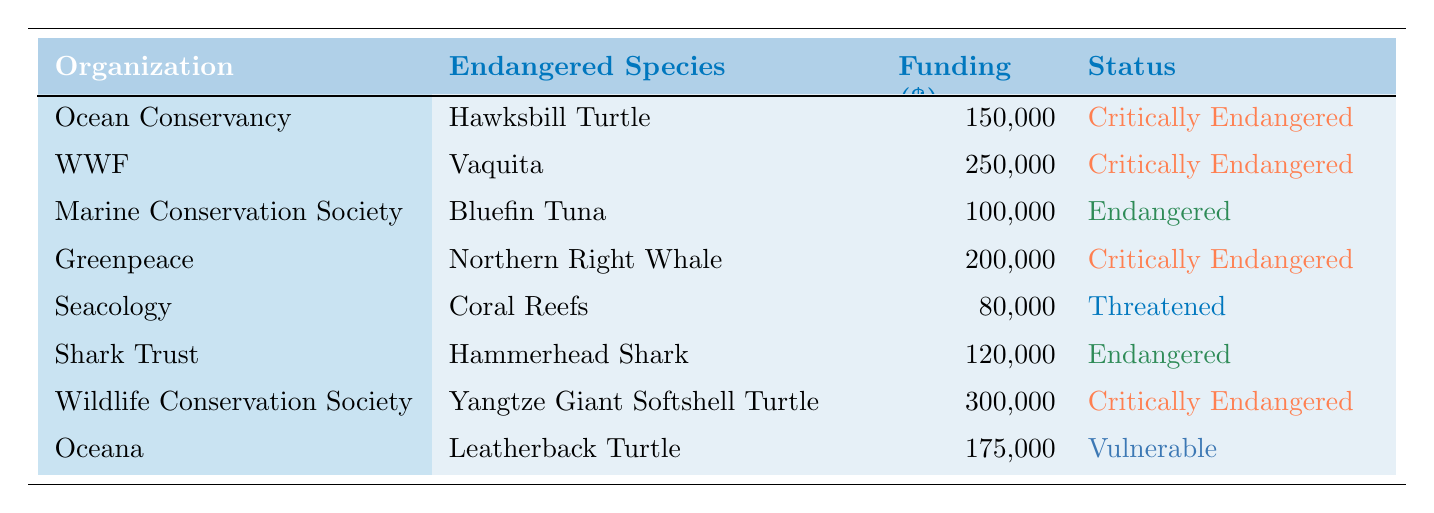
\begin{tikzpicture}

% Create the table using a matrix of nodes
\matrix (m) [matrix of nodes,
    nodes={
        anchor=west,
        inner xsep=6pt,
        inner ysep=5pt,
        text height=1.5ex,
        text depth=0.25ex,
        fill=rowblue % Default fill for data rows
    },
    row sep=-\pgflinewidth,
    column sep=-\pgflinewidth,
    % Header row style
    row 1/.style={nodes={
        fill=headerblue,
        font=\bfseries,
        text height=2ex,
        text depth=0.5ex,
        align=left
    }},
    % Column styles for data rows
    column 1/.style={nodes={text width=4.6cm, fill=orgblue}},
    column 2/.style={nodes={text width=5.3cm}},
    column 3/.style={nodes={text width=2.0cm, align=right}},
    column 4/.style={nodes={text width=3.7cm}},
    % Override alignment for header cells (redundant with row 1 style but explicit)
    row 1 column 1/.style={nodes={align=left, fill=headerblue}},
    row 1 column 2/.style={nodes={align=left}},
    row 1 column 3/.style={nodes={align=left}},
    row 1 column 4/.style={nodes={align=left}},
]
{
    % Header with specific text colors
    |[text=white]| Organization & |[text=headertextblue]| Endangered Species & |[text=headertextblue]| Funding (\$) & |[text=headertextblue]| Status \\
    % Data rows with specific text colors for the Status column
    Ocean Conservancy & Hawksbill Turtle & 150,000 & |[text=statuscritical]| Critically Endangered \\
    WWF & Vaquita & 250,000 & |[text=statuscritical]| Critically Endangered \\
    Marine Conservation Society & Bluefin Tuna & 100,000 & |[text=statusendangered]| Endangered \\
    Greenpeace & Northern Right Whale & 200,000 & |[text=statuscritical]| Critically Endangered \\
    Seacology & Coral Reefs & 80,000 & |[text=statusthreatened]| Threatened \\
    Shark Trust & Hammerhead Shark & 120,000 & |[text=statusendangered]| Endangered \\
    Wildlife Conservation Society & Yangtze Giant Softshell Turtle & 300,000 & |[text=statuscritical]| Critically Endangered \\
    Oceana & Leatherback Turtle & 175,000 & |[text=statusvulnerable]| Vulnerable \\
};

% Draw the horizontal lines
\draw (m.north west) -- (m.north east);
\draw (m-1-1.south west) -- (m-1-4.south east);
\draw (m.south west) -- (m.south east);

\end{tikzpicture}
\end{document}
